% Zadnja posodobitev: 25. 1. 2015
\documentclass[twoside,11pt]{article}
\usepackage[slovene]{babel}
\usepackage[utf8]{inputenc}
\usepackage{graphicx}
\usepackage[frame]{matrika}
\usepackage{mathtools}
\usepackage{epstopdf}
%\usepackage{amsmath,amssymb,amsfonts}
\usepackage{url}
\usepackage{enumitem}

% za stevilske mnozice uporabi naslednje simbole
\newcommand{\R}{\mathbb R}
\newcommand{\N}{\mathbb N}
\newcommand{\Z}{\mathbb Z}
\newcommand{\C}{\mathbb C}
\newcommand{\Q}{\mathbb Q}

\newcommand{\graf}[1][G]{\ensuremath{#1 = (V(#1), E(#1))}}

% operatorji
\DeclareMathOperator {\stopnja} {deg}
\DeclareMathOperator {\id} {id}
\DeclareMathOperator {\X}{X}
\DeclareMathOperator{\distance}{d}

% Po potrebi se lahk dodajo drugi standardni paketi, ki ne spreminjajo izgleda dokumenta


\begin{document}

\MAT{~}{1}{2016}

\naslov{Problem londonskega stolpa}

\avtor{Ines Meršak}

\institucija{Fakulteta za matematiko in fiziko \\ Univerza v Ljubljani}

\klasifikacija{~} 
\izvlecek{Problem londonskega stolpa je miselna uganka; dane imamo palice določenih višin, na katerih so razporejene krogle različnih barv. Cilj igre je s čim manj premiki krogel preiti iz začetnega stanja v neko končno (dano) stanje krogel. Za tak problem lahko narišemo graf, pri čemer so stanja krogel vozlišča, veljavne poteze pa povezave. V nalogi obravnavamo lastnosti tega grafa -- najprej za klasični problem londonskega stolpa, kjer imamo $3$ palice (višin $1$, $2$, $3$) in 3 krogle različnih barv, nato pa še za splošen primer s $p$ palicami in $n$ kroglami. Izkaže se, da je graf klasičnega problema ravninski in vsebuje Hamiltonovo pot, ni pa Hamiltonov. Pri splošnem primeru dokažemo, da je graf nekega problema londonskega stolpa povezan natanko tedaj, ko lahko krogle razporedimo tako, da najvišja palica ostane prazna. Prav tako ugotovimo, da so ravninski le grafi problemov z dvema kroglama in nekateri grafi problemov s tremi kroglami. V nalogi obravnavamo tudi poseben primer londonskega stolpa, pri katerem so vse palice enake višine $n$, imenovan oxfordski stolp. Za tak problem izpeljemo formulo za število vozlišč in povezav za poljubna $n$ in $p$. Na koncu se dotaknemo tudi simetrij grafa nekega problema londonskega stolpa in na primeru demonstriramo, kako lahko z upoštevanjem teh simetrij bolj učinkovito določimo predvsem metričnih lastnosti teh grafov.}
\title{The Tower of London problem}
\abstract{The Tower of London is a problem-solving puzzle, which consists of pegs of various heights that hold different-coloured balls of the same size. The aim of the puzzle is to get from the beginning state of the balls to the given end state with as little moves as possible. In order to study this problem, we use graph theory: a graph of the problem, called the London graph, can be drawn. Here, the vertices of the graph are all possible states and the edges are valid moves between these states. In this work, we take a look at some of the properties of London graphs. First, we analyse the graph of the classical (Shallice's) version of the problem, which consists of $3$ balls and $3$ pegs (of heights $1$, $2$, $3$, respectively), which turns out to be planar and contains a Hamiltonian path, but is not Hamiltonian.
After that, we take a look at the graph of the generalized Tower of London with $n$ balls and $p$ pegs. We prove that such a graph is connected if and only if the balls can be rearranged in a way that the tallest peg remains empty. Furthermore, we find that only  the problems with two balls (and some of those with three balls) have planar graphs. In this work, we also take a look at a special case of the Tower of London called the Tower of Oxford, where all the pegs are of the same height $n$. We prove an explicit formula to calculate the number of vertices and edges of the Oxford graph for all $n$ and $p$. In the end, we touch upon the symmetries of the London graphs and demonstrate how we can take advantage of them in order to calculate some metric properties more effeciently.}

\glava\baselineskip=14.5pt

\smallskip

\section{Uvod}

Test londonskega stolpa je ena izmed variacij Hanojskih stolpov. Izumil ga je britanski nevropsiholog Tim Shallice leta 1982 \cite{bib:wikishal}, da bi služil kot pripomoček pri ugotavljanju stanja pacientove psihe, in ocenjevanju napredka nekaterih bolezni, npr.\ Parkinsonove in Alzheimerjeve bolezni.  Uporablja se še danes, zato si bomo pogledali nekaj teorije tega problema, ki lahko pripomore k načrtovanju bolj ustreznih psiholoških testov. 

Osnovna verzija londonskega stolpa vsebuje tri enako velike krogle različnih barv in tri palice. Na prvo palico lahko postavimo samo eno kroglo, na drugo le dve krogli, na tretjo pa tri. Cilj igre je priti iz nekega danega stanja v neko drugo želeno stanje s čim manj potezami. Ta problem lahko elegantno analiziramo s pomočjo teorije grafov.

Članek je razdeljen na dva dela: v prvem delu si bomo podrobneje ogledali klasični londonski stolp in lastnosti pripadajočega grafa, v drugem delu pa bomo obravnavali posplošeni problem londonskega stolpa. Če ne bo navedeno drugače, bomo črpali iz vira~\cite{bib:tohmyths}.

\section{Klasični problem londonskega stolpa}
Pri klasičnem londonskem stolpu imamo tri enako velike krogle različnih barv in tri palice različnih velikosti: na prvo lahko postavimo eno kroglo, na drugo dve, na tretjo pa tri (temu bomo rekli, da imajo palice višine 1, 2 in 3). Cilj igre je priti iz nekega začetnega stanja v neko vnaprej določeno končno stanje.

\begin{figure}[h]
    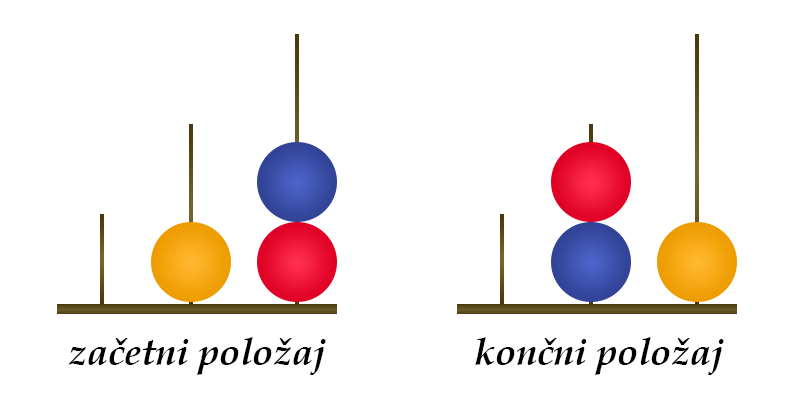
\includegraphics[width=250pt]{../img/london-tower.png}
    \caption{Na sliki sta prikazani dve možni stanji londonskega stolpa.}
    \label{fig:stanji}
\end{figure}

Stanja in prehode med njimi si najlažje predstavljamo, če narišemo graf. V ta namen vpeljemo naslednje oznake:
krogle bomo označili s številkami $1$, $2$, $3$ -- npr.\ modra krogla naj ima oznako $1$, rdeča $2$, rumena pa $3$ -- s simbolom ``$|$'' pa bomo označili konec prejšnje palice in začetek nove. Krogle bomo naštevali od vrha palice navzdol.

\begin{primer}
    Začetno stanje na sliki~\ref{fig:stanji} lahko torej opišemo z $|3|12$, končno stanje pa z $|21|3$.
\end{primer}
\medskip

S pomočjo teh oznak lahko opišemo vsako možno stanje in narišemo graf londonskega stolpa (označimo ga z $L$), pri čemer so vozlišča stanja, povezave pa so med tistimi stanji, med katerimi lahko prehajamo z eno potezo (enim veljavnim premikom krogle).

\begin{figure}[h!]
    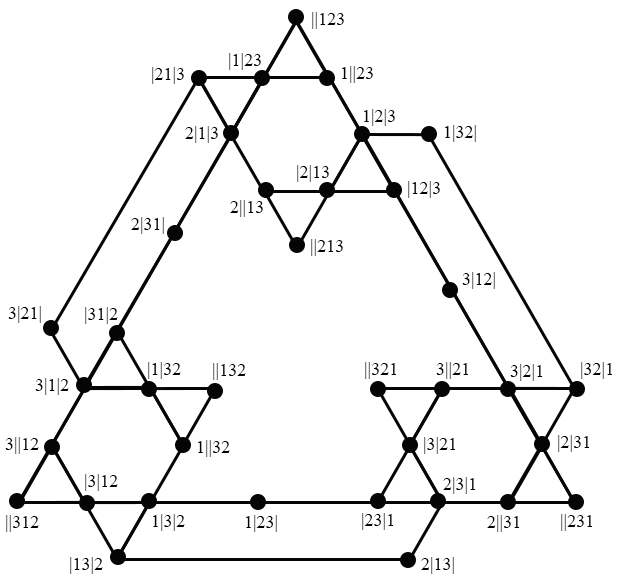
\includegraphics[width=300pt]{img/classic-tolgraph.png}
    \caption{Graf $L$ klasičnega Londonskega stolpa.}
    \label{fig:tolgraph}
\end{figure}

\begin{lema}
    \label{lem:stanja-klas-lond}
    Število vseh možnih stanj klasičnega londonskega stolpa je 36.
\end{lema}

%\proof
%Najprej si oglejmo vse možne postavitve krogel, pri čemer se ne oziramo na barvo.
%Imamo dve možnosti:
%\begin{enumerate}
%    \item \textbf{Na prvi (najkrajši) palici je krogla.}
%    Preostali dve krogli lahko razdelimo na drugi dve palici tako, da:
%    \begin{itemize}[label={-}]
%        \item je prazna druga palica,
%        \item je prazna tretja palica,
%        \item ima vsaka palica po eno kroglo.
%    \end{itemize}
%    Torej imamo v tem primeru tri možnosti.
%    
%    \item \textbf{Na prvi (najkrajši) palici ni krogle.}
%    Na drugi dve palici moramo torej razdeliti vse tri krogle.
%    Ponovno imamo tri možnosti:
%    \begin{itemize}[label={-}]
%        \item druga palica je prazna, tretja palica pa polna (na njej so tri krogle),
%        \item na drugi palici je ena krogla, na tretji palici pa dve krogli,
%        \item druga palica je polna (na njej sta dve krogli), na tretji palici pa je ena krogla.
%    \end{itemize}
%\end{enumerate}
%Po pravilu vsote imamo torej, če se ne oziramo na barve krogel, $3+3=6$ možnih postavitev krogel.
%V vsaki od teh lahko še premešamo barve krogel, torej imamo za vsako postavitev $3!$ možnosti. Sledi, da je vseh možnih stanj $3! \cdot 6 = 6 \cdot 6 = 36$.\qedhere
%\endproof

Iz leme~\ref{lem:stanja-klas-lond} sledi, da ima $L$ 36 vozlišč. Hitro vidimo, da je 12 vozlišč grafa $L$ stopnje 2, drugih 12 je stopnje 3, zadnjih 12 pa stopnje 4. 

\begin{primer}
    S pomočjo grafa na sliki~\ref{fig:tolgraph} lahko hitro ugotovimo, da za prehod med stanjema $|3|12$ in $|21|3$, ki sta prikazani na sliki~\ref{fig:stanji}, potrebujemo minimalno 4 poteze in da obstaja le eno najkrajše možno zaporedje potez.
\end{primer}

\bigskip

Preden preučimo še ostale lastnosti grafa klasičnega problema londonskega grafa, pa se spomnimo nekaj definicij. \emph{Premer} nekega grafa je definiran kot največja možna razdalja med poljubnima dvema paroma vozlišč v grafu. Premer bo pri našem problemu merilo težavnosti, saj nam bo povedal, s kakšnim številom potez je vedno mogoče priti od poljubnega začetnega do poljubnega končnega stanja.

Zanimali nas bosta tudi povezanost in ravninskost.
Graf je \emph{povezan}, če lahko najdemo pot med poljubnima dvema vozliščema v grafu. Če bo graf našega problema povezan, bo to pomenilo, da bo problem vedno rešljiv za poljubno kombinacijo začetnega in končnega stanja. 
Graf je \emph{ravninski}, če ga lahko narišemo v ravnini brez križanja povezav. Ker je londonski graf pri psiholoških testiranjih pogosto uporabljen za prikaz rezultata pacienta, bi križanje povezav lahko pripeljalo do zmede, zato si želimo, da bo graf našega problema ravninski.

Zanimalo pa nas bo tudi, ali graf vsebuje nek cikel, ki bi obšel vsa vozlišča grafa natanko enkrat. Takim grafom pravimo \emph{Hamiltonovi grafi}. Če pa lahko v grafu najdemo le pot, ki gre skozi vsa vozlišča, pa rečemo, da graf vsebuje Hamiltonovo pot.


Vrnimo se k grafu klasičnega problema londonskega stolpa. S pomočjo slike~\ref{fig:tolgraph} lahko vidimo, da je ravninski in ima premer $8$. Dokažemo pa lahko tudi spodnjo trditev.

\begin{trditev}
    Graf $L$ vsebuje Hamiltonovo pot, ne pa tudi Hamiltonovega cikla.
\end{trditev}

\begin{proof}
Hitro lahko dokažemo, da $L$ vsebuje Hamiltonovo pot: poiščemo jo. Ena izmed Hamiltonovih poti v grafu $L$ je prikazana na sliki~\ref{fig:dokaz-ham-klasicni} levo.

\begin{figure}
    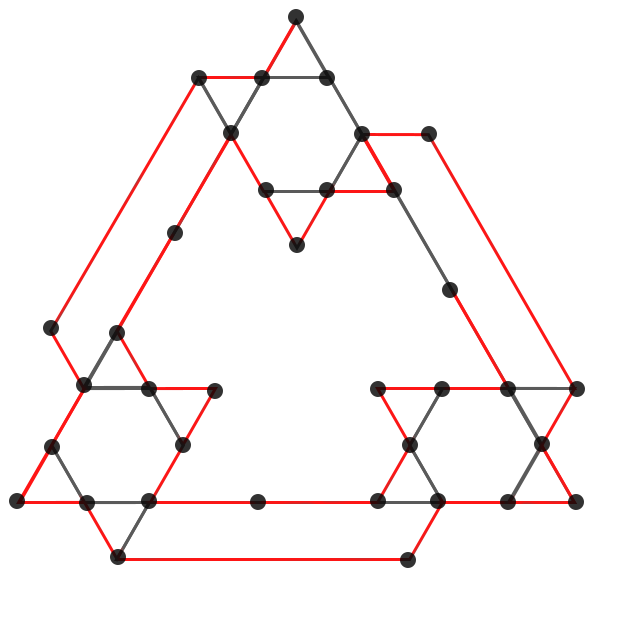
\includegraphics[width=210pt]{img/classic-tolgraph-ham-path.png}
    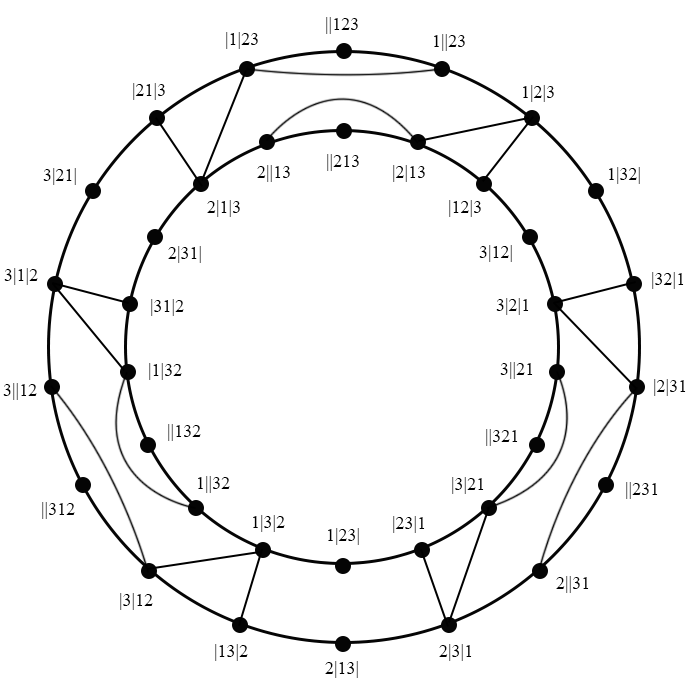
\includegraphics[width=210pt]{img/classic-tolgraph-hamcycle.png}
    \caption{Ena izmed Hamiltonovih poti v grafu $L$ (levo) in graf $L$ narisan malo drugače (desno).}
    \label{fig:dokaz-ham-klasicni}
\end{figure}

Da bi dokazali, da graf ni Hamiltonov, moramo najprej opaziti nekaj lastnosti tega grafa. Soseščina vsakega vozlišča stopnje $2$ je sestavljena iz enega vozlišča stopnje $3$ in enega stopnje $4$, prav tako je presek soseščin poljubnih dveh vozlišč stopnje $2$ prazen -- vsako vozlišče stopnje $2$ ima torej ``svoje'' vozlišče stopnje $3$ in stopnje $4$. Nadalje lahko iz grafa vidimo, da poljubni dve vozlišči stopnje $3$ nista sosednji.

Sledi, da na ciklu $C$ v grafu, ki bi vseboval vsa vozlišča, nobeni dve vozlišči stopnje $4$ nista sosednji. Ker imamo po $12$ vozlišč vsake stopnje, bi v nasprotnem primeru namreč prišli do zaključka, da morata biti sosednji dve vozlišči stopnje $3$, kar pa je v protislovju z zgornjim opažanjem.

Sedaj začnimo graditi cikel $C$, ki bo vseboval vsa vozlišča grafa natanko enkrat. Oglejmo si sliko~\ref{fig:dokaz-ham-klasicni} desno.
Cikel $C$ mora torej gotovo iti skozi vsa vozlišča stopnje $2$, kar je možno le na en način: če imamo vozlišče stopnje $2$ $v$ s sosedoma $u$ stopnje $3$ in $z$ stopnje $4$, mora $C$ vsebovati pot $u,v,z$.
Če začnemo pri vozlišču stopnje $2$ $||123$, mora graf torej vsebovati pot $1||23, ||123, |1|23$. Slednje je vozlišče stopnje $4$, za nadaljevanje cikla pa imamo dve možnosti: vozlišče $2|1|3$ ali $|21|3$. Ker je prvo stopnje $4$ in smo že prej opazili, da dve vozlišči enake stopnje ne bosta sosednji na ciklu $C$, cikel nadaljujemo z $|21|3$. Sosed tega vozlišča je vozlišče $3|21|$ stopnje $2$, zato moramo cikel gotovo nadaljevati skozi njega. Pridemo do vozlišča $3|1|2$. Imamo dve možnosti: 
\begin{itemize}[label={--}]
    \item Nadaljujemo z vozliščem $|31|2$, ki je stopnje $3$ in je na notranjem ciklu. V tem primeru ne bomo notranjega cikla nikoli zapustili, saj je notranji cikel oblike: vozlišče stopnje $2$, vozlišče stopnje $3$ (povezano samo z vozlišči na notranjem ciklu), vozlišče stopnje $4$, ki je nato povezano z vozliščem stopnje $2$, skozi katerega moramo iti. Nato pa sledita vozlišče $a$ stopnje $3$ (povezano z notranjim ciklom in vozliščem $w$ stopnje $4$ na zunanjem ciklu) in vozlišče $b$ stopnje $4$ (povezan z vozliščem $c$ stopnje $2$ in še dvema drugima na notranjem ciklu ter vozliščem $w$). Ker moramo iti skozi vozlišče $c$, moramo tudi skozi $b$, od prej pa vemo, da moramo nujno tudi skozi $a$, saj je sosed vozlišča stopnje $2$. Torej lahko pot speljemo le skozi $a,b,c$, saj je $w$ stopnje $4$ in na ciklu zato ne sme biti soseden $b$, ki je prav tako stopnje $4$.
    \item Pot torej nadaljujemo z vozliščem stopnje $3$ na zunanjem ciklu $3||12$, in tudi v nadaljevanju ostanemo na zunanjem ciklu, saj vemo, da bomo v nasprotnem primeru ostali na notranjem ciklu.
\end{itemize}
Ne moremo konstruirati cikla, bi vseboval vsa vozlišča našega grafa $L$ natanko enkrat, $L$ torej ni Hamiltonov.
\qedhere
\end{proof}

\section{Posplošeni londonski stolp}
Graf klasičnega problema londonskega stolpa je majhen, zato je za psihološka testiranja naloga včasih prelahka. 
Jenny R.\ Tunstall je prva predlagala razširitev klasičnega londonskega stolpa na 4 krogle s podaljšanimi palicami (vsaka je podaljšana za eno enoto), mi pa si bomo v tem razdelku pogledali ta problem v splošnem, s $p \geq 3$ palicami in $n \geq 2$ kroglami.

\subsection{Definicija}

Posplošen londonski stolp ima $n \geq 2$ krogel, označimo jih s številkami $1,\ldots,n$, in $p \geq 3$ palic, katerih višino označimo s $h_k$ -- toliko krogel lahko postavimo na $k$-to palico. Seveda velja, da mora biti število vseh krogel manjše ali enako vsoti višin vseh palic, sicer na palice ne moremo razporediti vseh krogel. S simboli zapišemo:
\[ n \leq \sum_{k=1}^{p} h_k.\]
Edina omejitev premikov krogel je ponovno višina palic, prav tako je enak cilj igre: priti iz začetnega stanja v končno stanje s čim manj premiki.

Pred definicijo splošnega londonskega grafa vpeljimo oznake, ki jih bomo uporabljali za opis stanja nekega splošnega londonskega stolpa. Enoličen zapis lahko dosežemo, če vsako stanje predstavimo s permutacijo $s$ iz simetrijske grupe $S_{n+p}$. Pri tem $i$-ta števka permutacije predstavlja

\[ s_i =
\begin{cases}
\text{položaj krogle } i, & i \in [n] \\
\text{položaj dna palice } i-n, & i \in [n+p] \setminus [n]
\end{cases},
\]
kjer $[n]$ označuje množico $\{1,2,\ldots, n \}$.

Položaje oštevilčimo od leve palice proti desni, z vrha palice proti dnu. Tako bo s številko $1$ oštevilčen položaj krogle, ki je postavljena najvišje na prvi palici; če na prvi palici ni nobene krogle, bo imelo položaj $1$ dno te palice.

\begin{primer}
    Poiščimo permutacijo za začetni položaj na sliki~\ref{fig:stanji}, ki smo ga označili z $|3|12|$. 
    Predstavljajmo si, da oštevilčujemo krogle in dna palice, in začnimo oštevilčevati od leve proti desni, z vrha palice proti dnu, tako kot je prikazano na sliki~\ref{fig:ostev-stanji}.
    
    \begin{figure}[h]
        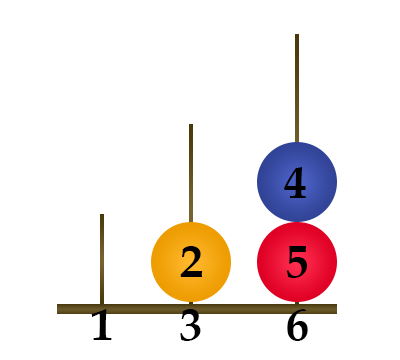
\includegraphics[width=220pt]{../img/london-tower-numbered.png}
        \caption{Položaji krogel in palic za stanje $|3|12|$.}
        \label{fig:ostev-stanji}
    \end{figure}
    
    Sedaj le preberemo položaje vseh krogel (od prve do tretje) in vseh palic (od leve proti desni) -- prva (modra) krogla je oštevilčena s 4, druga (rdeča) s 5, \ldots
    To stanje lahko torej predstavimo s permutacijo $s=452136$.
\end{primer}

Hitro vidimo, da mora veljati 
\[\forall k \in [p]\colon s_{n+k} - s_{n+k-1} \geq 1 \]
saj je $s_{n+k}$ položaj dna palice $k$, $s_{n+k-1}$ pa položaj dna palice $k-1$, torej se mora njun položaj razlikovati najmanj za 1 -- to se zgodi, če na palici $k$ ni nobene krogle.

Prav tako pa velja tudi 
\[\forall k \in [p]\colon s_{n+k} - s_{n+k-1} \leq h_k + 1,\]
kar se zgodi v primeru, če je na $k$-ti palici $h_k$ krogel.

Opazimo še, da je položaj dna zadnje palice $s_{n+p}$ vedno enak $n+p$, saj smo pred tem že oštevilčili položaje vseh $n$ krogel in ostalih $p-1$ palic.

V splošnem je londonski graf, katerega vozlišča so vsa stanja pripadajočega londonskega stolpa, torej smiselno definirati takole:

\begin{definicija}
    Za \emph{londonski graf} $L_h^n$, kjer je $p \geq 3,\ n \geq 2,\ h \in [n]^p,\  \sum_{k=1}^p h_k \geq n$ velja:
    \begin{itemize}
        \item vozlišča so vse permutacije $s \in S_{n+p}$, za katere velja:
        \[\forall k \in [p]:\ 1 \leq s_{n+k} - s_{n+k-1} \leq h_k + 1,\ s_{n+p} = n + p ,\]
        \item vsaki dve stanji (oz.\ pripadajoči permutaciji), med katerima lahko prehajamo z veljavno potezo, sta povezani.
    \end{itemize}
\end{definicija}

S pogojem, da so vse palice visoke največ $n$, ne izgubimo splošnosti, saj razporejamo le $n$ krogel.

Očitno je klasičen londonski graf $L$ enak $L_{123}^3$, saj imamo $3$ krogle in $3$ palice, ki so velikosti $1$, $2$ in $3$.
Če smo za ta primer lahko izračunali število vozlišč, pa je v splošnem za londonske stolpe to precej težko. V naslednjem podrazdelku bomo obravnavali poseben primer londonskih grafov, za katerega je znana formula za število vozlišč. 

\subsection{Oxfordski graf}

\emph{Oxfordski graf} je poseben primer londonskega grafa, za katerega velja, da so vse palice velikosti $n$, pri čemer je $n$ število krogel. Oxfordski graf označimo z $O^n_p$, zanj torej velja $O^n_p := L^n_{n^p}$.

Medtem ko je v splošnem težko določiti število vozlišč londonskega grafa, pa je to precej bolj preprosto za oxfordski graf. Še več, določimo lahko tudi število povezav.

\begin{trditev}
    Število vozlišč oxfordskega grafa $O^n_p$ je enako 
    \begin{equation}
    \label{eq:oxford-vozl}
    \frac{(n+p-1)!}{(p-1)!}.
    \end{equation}
    
\end{trditev}

\begin{proof}
Iščemo število vseh možnih stanj krogel oxfordskega stolpa, saj je to enako številu vozlišč oxfordskega grafa.
Podobno kot pri dokazu števila stanj klasičnega londonskega stolpa najprej pozabimo na različne barve krogel (pretvarjamo se, da so krogle enake) in se osredotočimo samo na njihovo postavitev. 

Na koliko načinov lahko $n$ enakih krogel razporedimo na $p$ palic višine $n$? Pri tem nimamo nobenih omejitev, saj so palice dovolj visoke, da lahko vse krogle postavimo tudi na eno samo palico. Lahko si predstavljamo, da imamo vse krogle zložene v vrsto, označene naj bodo z 0, nato pa na poljubna mesta (s ponavljanjem) vrivamo 1, ki naj pomeni konec neke palice in začetek neke druge. Ko vrinemo $p-1$ enic, smo določili $p$ palic in s tem razporeditev krogel. 

Sedaj lahko na problem pogledamo malo drugače: na $n+p-1$ mest razporejamo $n$ ničel, ki predstavljajo krogle, in $p-1$ enic, ki predstavljajo začetek nove palice. Če razporedimo vse enice, bodo vsa preostala mesta zasedle ničle, razporeditev bo s tem točno določena. Načinov za izbiro $p-1$ mest za enice izmed $n+p-1$ položajev je ${n+p-1 \choose p-1}$. Če privzamemo, da so vse krogle enake, je vseh možnih razporeditev torej ${n+p-1 \choose p-1}$.

Ker je vsaka krogla drugačne barve, imamo za vsako razporeditev še $n!$ možnih permutacij barv. Število vseh stanj, in zato tudi število vozlišč, je tako enako

\[ n! \cdot {n+p-1 \choose p-1} = n! \cdot \frac{(n+p-1)!}{n!(p-1)!} = \frac{(n+p-1)!}{(p-1)!}. \] \qedhere
\end{proof}

\begin{trditev}
    Število povezav oxfordskega grafa $O^n_p$ je enako
    \begin{equation}
    \label{eq:povezave-oxf}
    \frac{np}{2} \frac{(p-2+n)!}{(p-2)!}
    \end{equation}
    \label{trd:povezave-oxf}
\end{trditev}

Preden si ogledamo izpeljavo formule~\eqref{eq:povezave-oxf}, pa si na hitro oglejmo še sledečo lemo, ki jo bomo potrebovali pri dokazu.

\begin{lema}
    Velja naslednja lastnost binomskih simbolov:
    \begin{equation}
    \label{eq:binom}
    {b+w \choose l} = \sum_{k=0}^{l}{b \choose k}{w \choose l-k}.
    \end{equation}
\end{lema}

To lemo lahko hitro dokažemo s preprostim kombinatoričnem razmislekom, vendar bomo dokaz zaradi jedrnatosti izpustili. Spomnimo pa se še leme o rokovanju:
\begin{lema}[Lema o rokovanju]
    \label{lema:rokovanje}
    Za vsak graf \graf velja formula
    \begin{equation}
    \sum_{u \in V(G)}\! \stopnja u = 2 \cdot |E(G)|.
    \label{eq:lema-o-rokovanju}
    \end{equation}
\end{lema}

Sedaj imamo vse, kar potrebujemo za dokaz trditve o številu povezav oxfordskih grafov.

\proof[Dokaz trditve~\ref{trd:povezave-oxf}]
Vzemimo stanje (vozlišče) s $q$ nepraznimi palicami, pri čemer je $q$ fiksen ter velja $1 \leq q \leq p$ in $n \geq q$. Preštejmo vse veljavne poteze, ki jih lahko naredimo ob takem stanju krogel. Vsako vrhnjo kroglo ene izmed $q$ palic lahko premaknemo na katerokoli palico, razen trenutne; izberemo torej eno izmed $q$ palic, s katere premaknemo kroglo, in eno izmed preostalih $p-1$ palic, kamor kroglo premaknemo. Tako vozlišče je torej stopnje $q(p-1)$. (Pri tem upoštevamo, da je povezava med dvema vozliščema grafa pravzaprav veljavna poteza med dvema stanjema.)

Ugotovili smo, da so vsa stanja oziroma pripadajoča vozlišča, ki imajo točno $q$ nepraznih palic, enake stopnje. Ker želimo uporabiti lemo o rokovanju, moramo najprej prešteti, koliko je takih stanj. 
Izberemo $q$ izmed $p$ palic, ki bodo neprazne, kar lahko storimo na ${p \choose q}$ načinov. Na vsako izmed teh $q$ palic moramo nujno postaviti vsaj eno kroglo, kar lahko naredimo na $n \cdot (n-1) \cdot \ldots \cdot (n-q+1) = \frac{n!}{(n-q)!}$ (za prvo izmed $q$ palic imamo na voljo $n$ krogel, za drugo $n-1$ krogel,\ldots). S tem zagotovimo, da je točno $q$ palic res nepraznih. Preostalih $n-q$ krogel pa lahko razporedimo poljubno na $q$ palic, kar je brez škode za splošnost enako številu razporeditev $n-q$ krogel na $q$ palic velikosti $n-q$, torej $|V(O^{n-q}_q)|$.
Iz tega razmisleka sledi, da je število vseh stanj, ki imajo točno $q$ nepraznih palic, torej enako
\[{p \choose q} \frac{n!}{(n-q)!} \cdot |V(O^{n-q}_q)|.\]
Če uporabimo še formulo za število vozlišč oxfordskega grafa~\eqref{eq:oxford-vozl} in poračunamo, dobimo, da je število takih stanj enako
\begin{align*}
{p \choose q} \frac{n!}{(n-q)!} \cdot |V(O^{n-q}_q)| &=
{p \choose q} \frac{n!}{(n-q)!} \frac{(n-q+q-1)!}{(q-1)!} \\ &= n! {p \choose q} \frac{(n-1)!}{(q-1)!\,(n-q)!} \\ &=
n! {p \choose q} {n-1 \choose q-1}
\end{align*}

Sedaj po $q$ seštejemo stopnje vseh vozlišč (upoštevamo, da imajo vsa vozlišča, kjer je nepraznih točno $q$ palic, enako stopnjo) in uporabimo formulo~\eqref{eq:lema-o-rokovanju} iz leme o rokovanju:
\begin{align*}
|E(O^n_p)|
&= \frac{1}{2} \sum_{q=1}^{p} \overbrace{q(p-1)}^{\text{stopnja vozlišča}} 
\overbrace{n! {p \choose q} {n-1 \choose q-1} }^{\text{št.~vozlišč s to stopnjo}} \\
&= \frac{1}{2} (p-1) n! \sum_{q=1}^{p} q {p \choose q} {n-1 \choose q-1} \\
&= \frac{1}{2} (p-1) n! \sum_{q=1}^{p} q \frac{p!}{q! \, (p-q)!} {n-1 \choose q-1} \\
&= \frac{1}{2} (p-1) n! \sum_{q=1}^{p} p \frac{(p-1)!}{(q-1)! \, (p-q)!} {n-1 \choose q-1} \\
&= \frac{1}{2} p (p-1) n! \sum_{q=1}^{p} {p-1 \choose q-1} {n-1 \choose q-1}
\end{align*}
Sedaj uvedemo nov indeks $k = q-1$, upoštevamo lastnosti binomskih simbolov in uporabimo zgoraj dokazano formulo~\eqref{eq:binom}:
\begin{align*}
|E(O^n_p)|
&= \frac{1}{2} p (p-1) n! \sum_{k=0}^{p-1} {p-1 \choose k} {n-1 \choose k} \\
&= \frac{1}{2} p (p-1) n! \sum_{k=0}^{p-1} {p-1 \choose p-1-k} {n-1 \choose k} \\
&= \frac{1}{2} p (p-1) n! {p-1 + n-1 \choose p-1} \\
&= \frac{1}{2} p (p-1) n! {n + p - 2 \choose p-1} \\
&= \frac{1}{2} p (p-1) n! \frac{(n+p-2)!}{(p-1)!\,(n-1)!} \\
&= \frac{1}{2} p n \frac{(n+p-2)!}{(p-2)!} \\
&= \frac{np}{2} \frac{(p-2+n)!}{(p-2)!} \qedhere
\end{align*}
\endproof

\subsection{Povezanost}

Zaželjeno je, da lahko pri londonskem stolpu, s pomočjo katerega opravljajo teste v psihologiji, prehajamo med poljubnima dvema stanjema. To velja, če je pripadajoči londonski graf povezan, kar je zato ena pomembnejših lastnosti tega grafa.
V nadaljevanju bomo privzeli, da so palice urejene po velikosti naraščajoče, velja torej $h_1 \leq h_2 \leq \cdots \leq h_p$.
Potreben pogoj za povezanost londonskega grafa je očitno 
\[ n \leq \sum_{k=1}^{p-1} h_k, \]
oziroma z besedami, da lahko krogle razporedimo tako, da najvišja palica ostane prazna. V nasprotnem primeru bi, potem ko bi razporedili maksimalno možno število krogel na vse preostale (manjše) palice, na največji ostalo še nekaj krogel, ki jih nikoli ne bi mogli premakniti na kakšno drugo palico.
Izkaže se, da je ta pogoj tudi zadosten za povezanost londonskega grafa.

\begin{izrek}
    Londonski graf $L_h^n$ je povezan natanko tedaj, ko velja pogoj
    \begin{equation}
    n \leq \sum_{k=1}^{p-1} h_k.
    \label{eq:pogoj-povezanosti}
    \end{equation}
\end{izrek}

\proof
Želimo dokazati, da iz pogoja \eqref{eq:pogoj-povezanosti} sledi, da lahko najdemo pot med poljubnima dvema vozliščema v londonskem grafu, kar je ravno definicija povezanosti. Dokaza se lotimo tako, da najprej čim bolj zreduciramo splošen problem in nato rešimo zreduciran problem.

Spomnimo se, da vsako vozlišče londonskega grafa predstavlja neko stanje krogel -- če torej iščemo pot v grafu med dvema vozliščema, pravzaprav rešujemo problem, kako iz začetnega stanja krogel priti v končno. Fiksirajmo poljubno začetno in končno stanje in poskusimo rešiti ta problem.

Predpostavili bomo, da je število vseh krogel kar enako vsoti višin vseh palic brez največje, saj lahko v nasprotnem primeru vpeljemo navidezne krogle, katerih premike kasneje zanemarimo. Velja naj torej $n = \sum_{k=1}^{p-1}h_k$.

Nadalje lahko predpostavimo, da so krogle pri začetnem kot tudi pri končnem stanju razporejene tako, da je največja palica prazna. V nasprotnem primeru jih lahko na začetku razporedimo na preostale palice, na koncu pa preprosto prestavimo na največjo palico.

Torej je za dokaz povezanosti grafa dovolj, če najdemo pot med poljubnima dvema stanjema, pri katerem so vse palice (razen največje) zapolnjene, največja palica pa je prazna.

Sedaj postopamo tako, da izberemo kroglo, ki še ni na svojem (končnem) položaju, in jo zamenjamo s kroglo, ki se trenutno nahaja na tem položaju; ta postopek ponavljamo. Če lahko zamenjavo naredimo tako, da se pri tem ne spremeni položaj nobene druge krogle, je po koncu zamenjave še ena krogla več na pravem mestu.
Ker je največja palica prazna, vse druge pa zapolnjene, se po koncu ponavljanja tega postopka ne more zgoditi, da je le ena krogla (označimo jo z $a$) na napačnem mestu. V nasprotnem primeru bi zaradi zapolnjenosti palic namreč obstajala krogla $b$, ki bi bila na končnem mestu krogle $a$ in zato $b$ ne bi bila na svojem končnem položaju -- torej imamo vedno vsaj dve krogli, ki sta na napačnem mestu, ti dve krogli pa lahko spet zamenjamo.

Če torej dokažemo, da lahko poljubni dve krogli zamenjamo tako, da se pri tem ne spremeni položaj nobene druge krogle, bomo s ponavaljanjem zgornjega postopka lahko prešli iz začetnega v končno stanje krogel, graf bo povezan.

Sedaj predpostavimo še, da je ena izmed krogel, ki ju bomo zamenjali, na vrhu prve, najmanjše, palice. Namreč, s tremi zamenjavami, pri katerih je ena izmed krogel vedno na vrhu prve palice, lahko nadomestimo splošno zamenjavo dveh poljubnih krogel. Recimo, da želimo zamenjati poljubni krogli $a$ in $b$. Če uporabimo notacijo klasičnega problema, s $c$ označimo vrhnjo kroglo prve palice, z $x$ pa poljubno število nekih poljubnih krogel in če izpustimo palice, ki na to menjavo ne bodo imele vpliva, lahko menjavo $a$ in $b$ opravimo takole:

\[ cx|xax|xbx| \rightarrow bx|xax|xcx| \rightarrow ax|xbx|xcx| \rightarrow cx|xbx|xax|. \]

Pri tem je bila v vsaki menjavi udeležena vrhnja krogla prve palice.
Dovolj je torej dokazati, da lahko naredimo menjavo vrhnje krogle prve palice in neke druge poljubne krogle, brez da bi pri tem pokvarili položaj ostalih krogel.

Sedaj si izberimo kroglo, ki ni na pravem položaju, in s tem tudi kroglo, ki je trenutno na njenem položaju. Predpostavili smo, da je ena izmed teh krogel na prvi palici -- to kroglo označimo z $a$, drugo pa z $b$. Ločimo dva primera:

\begin{enumerate}
    \item \textbf{Krogla $b$ je na prvi palici.}
    Vrhnjo kroglo druge palice, označimo jo s $c$, premaknemo na največjo ($p$-to) palico. Nato kroglo $a$ premaknemo na vrh druge palice, preostale krogle na prvi palici z do vključno kroglo $b$ pa premaknemo (seveda eno naenkrat) na največjo palico. Krogla $a$ lahko sedaj zasede svoj pravi položaj na prvi palici, $b$ pa premaknemo iz vrha največje palice na vrh druge. Sedaj lahko vrnemo vse preostale krogle (razen $c$) na prejšnje mesto na prvi palici, nato lahko na vrh prve palice postavimo $b$, ki tako zavzame prejšnji položaj krogle $a$. Za konec premaknemo še kroglo $c$ z največje palice na vrh druge palice.
    \item \textbf{Krogla $b$ ni na prvi palici.}
    V tem primeru je postopek še nekoliko lažji: najprej vse krogle nad $b$ premaknemo na največjo palico, nato na vrh največje palice premaknemo tudi $b$. Sedaj lahko kroglo $a$ prestavimo na njeno pravo mesto (kjer je bil prej $b$), $b$ na vrh prve palice, vse preostale krogle na največji palici pa postavimo nazaj na prejšnja mesta, nad kroglo $a$.
\end{enumerate}
S tem je dokaz končan, saj smo našli način, kako prehajati med dvema poljubnima stanjema krogel, in smo s tem našli tudi pot v grafu med poljubnima vozliščema.
\endproof

\subsection{Ravninskost}

Povedali smo že, da se problem londonskega stolpa pogosto uporablja kot psihološki test. Psihologi rezultate testov radi prikažejo kar na grafu uporabljenega problema, zato je zanimivo tudi vprašanje ravninskosti londonskih grafov -- križanje povezav namreč lahko vodi do zmede pri prikazu rezultatov. Ker se za testiranje uporablja le londonski stolp s tremi palicami, se bomo tudi pri obravnavi ravninskosti omejili na ta primer, torej naj bo $p=3$.

Spomnimo se izreka, ki nam bo pomagal pri klasifikaciji ravninskih grafov. Dokaz bomo zaradi jedrnatosti in dolžine izpustili, naveden pa je v~\cite[str.~247-251]{bib:west}.

\begin{izrek}[Kuratowski]
    \label{izr:kuratowski}
    Graf G je ravninski natanko tedaj, ko ne vsebuje subdivizije $K_5$ niti subdivizije $K_{3,3}$.
\end{izrek}

Pri tem je \emph{subdivizija} sledeča operacija, ki ohranja ravninskost grafa: vzamemo neko povezavo grafa in na sredino te povezave dodamo še eno vozlišče (ta postopek lahko ponavljamo). \cite[str.~66]{bib:potocnik}

Najprej obravnavajmo primer londonskega stolpa z dvema kroglama ($n=2$, to so torej grafi $L^2_h$). V tem primeru imamo grafe 
$L^2_{111}, L^2_{112}, L^2_{122}$ in $L^2_{222} = O^2_3$ (še vedno predpostavljamo, da so palice razvrščene po velikosti naraščajoče). Hitro lahko vidimo, da je npr.\ $L^2_{111}$ podgraf $L^2_{112}$: iz prvega lahko pridemo do drugega tako, da dodamo vozlišči, kjer sta obe krogli na največji palici, in ustrezno dodamo povezave z že obstoječimi stanji. Če s $ \subset $ označimo relacijo podgraf, lahko vidimo sledeče:
\[ L^2_{111} \subset L^2_{112} \subset L^2_{122} \subset L^2_{222} = O^2_3 .\]
S slike~\ref{fig:graf-2krogli}, na kateri je narisan graf $O^2_3$, lahko zaključimo, da je ta graf ravninski. Iz tega seveda sledi, da so ravninski tudi vsi njegovi podgrafi, saj z brisanjem vozlišč in povezav ne moremo ustvariti križanj povezav. Torej so vsi londonski grafi za $n=2$ in $p=3$ ravninski.
Na sliki~\ref{fig:graf-2krogli} so pravzaprav prikazani grafi vseh londonskih stolpov z dvema kroglama -- rdeča barva označuje najmanjši graf, $L^2_{111}$, nato pa z zaporednim dodajanjem vozlišč in povezav dobimo še ostale: če dodamo zelena vozlišča, dobimo $L^2_{112}$, če nato dodamo še modra vozlišča, dobimo $L^2_{122}$; celoten graf pa (kot že omenjeno) predstavlja $O^2_3$ .

\begin{figure}[h]
    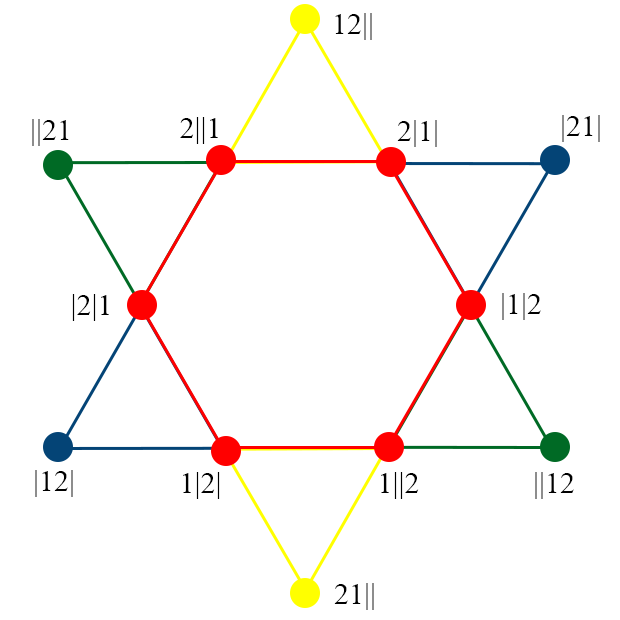
\includegraphics[width=170pt]{img/tolgraph-2balls.png}
    \caption{Vsi londonski grafi s $p=3$ in $n=2$ so ravninski.}
    \label{fig:graf-2krogli}
\end{figure}

Če si sedaj pogledamo problem londonskega stolpa s tremi kroglami ($n=3$), na podoben način kot za dve krogli dobimo sledečo shemo:

\begin{equation}
\label{eq:grafi-3krogle}
\begin{matrix}
& & L & & & & \\
& & \parallel & & & & \\
L_{122}^3 & \subset & L_{123}^3 & \subset & L_{133}^3 & & \\
\cap & & \cap & & \cap & & \\
L_{222}^3 & \subset & L_{223}^3 & \subset & L_{233}^3 & \subset & L_{333}^3 \\
& & & & & & \parallel \\
& & & & & & O^3_3 \\
\end{matrix}
\end{equation}

\smallskip

Videli smo že, da je klasični londonski graf $L$ ravninski. Torej je ravninski tudi njegov podgraf $L_{122}^3$, saj do njega pridemo tako, da iz $L$ zbrišemo tistih šest vozlišč, kjer so vse tri krogle na največji palici, in pripadajoče povezave. 
Če pa grafu $L$ dodamo vozlišča, kjer so vse tri krogle na srednji palici, lahko s slike~\ref{fig:L^3_133} vidimo, da je tudi $L_{133}^3$ ravninski (dodana vozlišča so označena z rdečo barvo).

\begin{figure}[h]
    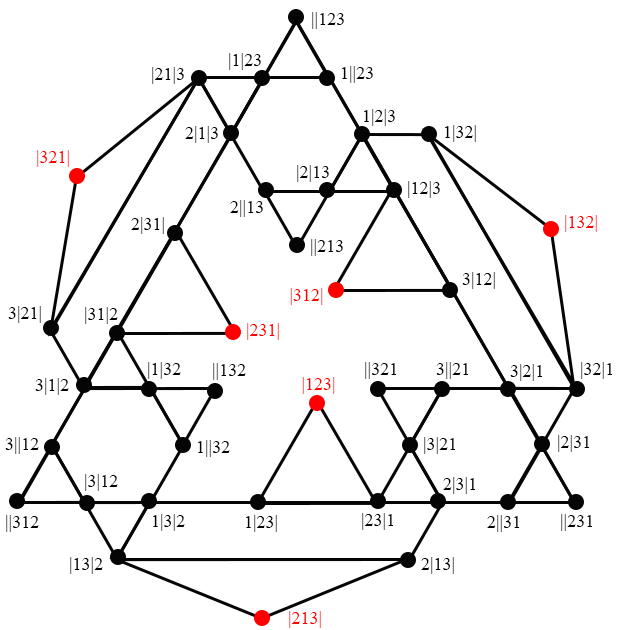
\includegraphics[width=350pt]{img/L_133.png}
    \caption{Graf $L^3_{133}$ je ravninski.}
    \label{fig:L^3_133}
\end{figure}

\begin{trditev}
    Naj bo $p=3$. Tedaj so ravninski londonski grafi natanko grafi $L_h^2, L_{122}^3, L_{123}^3$ in $L_{133}^3$.
\end{trditev}

\begin{opomba}
    Še vedno predpostavljamo, da so londonski grafi povezani, torej zadostujejo pogoju~\eqref{eq:pogoj-povezanosti}.
\end{opomba}

\proof[Oris dokaza.]
Videli smo že, da so grafi $L_h^2, L_{122}^3, L_{123}^3$ in $L_{133}^3$ ravninski. Dokazati moramo, da vsi ostali grafi za $n=3$ in vsi grafi za $n \geq 4$ niso ravninski, pri tem nam je v pomoč izrek Kuratowskega. Poiskati bi morali subdivizijo $K_{3,3}$ v grafu $L_{222}^3$, kar pa bomo tukaj izpustili in predpostavili, da ta graf res vsebuje subdivizijo $K_{3,3}$. Od tu sledi, da $L_{222}^3$ ni ravninski. Ker vsi preostali grafi z $n = 3$ vsebujejo graf $L_{222}^3$ (kot lahko vidimo na shemi~\eqref{eq:grafi-3krogle}), tudi $L_{223}^3, L_{233}^3, L_{333}^3=O^3_3$ niso ravninski.

Dokazati moramo le še, da tudi londonski grafi za $n\geq 4$ niso ravninski.
Ker $L_{222}^3$ ni ravninski in je vsebovan v grafu $L_{222}^4$, sledi, da $L_{222}^4$ ni ravninski. Pokazali bi lahko, da tudi graf $L_{133}^4$ ni ravninski, vendar si pri tem ne moremo pomagati z njegovim ravninskim podgrafom $L_{133}^3$, zato bi morali znotraj $L_{133}^4$ poiskati subdivizijo $K_{3,3}$, kar bomo prav tako izpustili.
Ker mora vsak graf $L_h^4$ vsebovati ali $L_{133}^4$ ali $L_{222}^4$, ki nista ravninska, to sledi tudi za preostale grafe z $n=4$.

Za $n \geq 4$ torej noben graf ni ravninski, saj vsak $L_h^n$ dobimo z dodajanjem krogel enemu izmed $L_h^4$, za katere pa zdaj vemo, da niso ravninski.
\endproof

?? Dragonhack Č=


\begin{thebibliography}{99}
\bibitem{bib:tohmyths} A.\ M.\ Hinz, S.\ Klavžar, U.\ Milutinović in C.\ Petr, \emph{The Tower of Hanoi – Myths and Maths}, Birkhäuser, Basel, 2013.

\bibitem{bib:west} D.\ B.\ West et al, \emph{Introduction to graph theory}, Prentice hall, Upper Saddle River, 2001.

%\bibitem{bib:tolspatial}
%W. K. Berg in D. L. Byrd, \emph{The Tower of London spatial problem-solving task: Enchancing clinical and research implementation}, Journal of Clinical and Experimental Neuropsychology \textbf{24} (2002) 586--604,
%dostopno tudi na \\ \url{https://www.researchgate.net/publication/11201010_The_Tower_of_London_Spatial_Problem-Solving_Task_Enhancing_Clinical_and_Research_Implementation}.
%
%\bibitem{bib:potocnik} P. Potočnik, \emph{Zapiski predavanj iz Diskretne Matematike I}, 1.~izdaja, [ogled 29.~12.~15], dostopno na \url{http://www.fmf.uni-lj.si/~potocnik/Ucbeniki/DM-Zapiski2010.pdf}.
%
%\bibitem{bib:wikishal} \emph{Tim Shallice}, v: Wikipedia: The Free Encyclopedia, [ogled 8.~10.~2015], dostopno na\\ \url{https://en.wikipedia.org/wiki/Tim_Shallice}.
%
%\bibitem{bib:wikihamilpath} \emph{Hamiltonian path}, v: Wikipedia: The Free Encyclopedia, [ogled 28.~12.~2015], dostopno na \url{https://en.wikipedia.org/wiki/Hamiltonian_path}.

\bibitem{7} E.A. Cornell, C.E. Wieman, M.R. Matthews, J.R. Ensher in M.H. Anderson, \emph{Observation of Bose-Einstein Condensation in a Dilute Atomic Vapor}, Science \textbf{269} (1995), 198--201. 
\bibitem{6} W. Ketterle, D.M. Kurn, D.S. Durfee, N.J. van Druten, M.R. Andrews, M.-O. Mewes in K.B. Davis, \emph{Bose-Einstein Condensation in a Gas of Sodium Atoms}, Physics Review Letters \textbf{75} (1995), 3969--3973. 
\bibitem{3} J. Klaers, J. Schmitt, F. Vewinger in M. Weitz, \emph{Bose-Einstein condensation of photons in an optical microcavity}, Nature \textbf{468} (2010), 545--548. 
\bibitem{10} T. Giamarchi, C. R\"uegg in O. Tchernyshyov, \emph{Bose-Einstein condensation in magnetic insulators}, Nature Physics \textbf{4} (2008), 198--204. 
\bibitem{1} J.F. Annett, \emph{Superconductivity, Superfluids and Condensates}, Oxford University Press, 2004.
\bibitem{8} L. Lewin, \emph{Polylogarithms and Associated Functions}, Elsevier Science Ltd., 1981. 
\bibitem{9} H. Wagner in N.D. Mermin, \emph{Absence of Ferromagnetism or Antiferromagnetism in One- or Two-Dimensional Isotropic Heisenberg Models}, Physics Review Letters  \textbf{17} (1996), 1133--1136.
\bibitem{2} J. Klaers, F. Vewinger in M. Weitz, \emph{Thermalization of a two-dimensional photonic gas in a ‘white-wall’ photon box}, Nature Physics \textbf{6} (2010), 512--515.

\end{thebibliography}

\end{document}
